\section{Métrique d'évaluation d'algorithmes de compression d'images}

Nous avons vu plusieurs algorithmes pour la compression des images. Il devient alors nécessaire d'introduire différentes métriques pour quantifier les différences entre l'image originale et celles compressées par les algorithmes.

Nous verrons dans cette partie différentes métriques, certaines pour quantifier les différences purement mathématiques et 
d'autres pour approximer les différences perceptibles par l'\oe il humain. Ces métriques seront utiles afin de déterminer plus tard 
le taux de compression optimal pour faire un compromis entre la taille du fichier et la qualité de l'image.

\subsection{Erreur Moyenne Quadratique}
Une première métrique permettant de quantifier la compression est l'\textbf{erreur moyenne quadratique (MSE)}. Cette métrique est très utilisée, notamment dans le domaine de l'apprentissage automatique. Elle mesure la moyenne des distances carrées entre la valeur initiale et la nouvelle valeur.
$$MSE = \frac{1}{3MN} \sum_{c \in \{r,g,b\}}\sum_{i=0}^{M-1} \sum_{j=0}^{N-1} (I_O^c(i,j)- I_C^c(i,j))^2$$
où $M$ et $N$ représentent respectivement la hauteur et la largeur de l'image, 
$I_O^c(i,j)$ (resp. $I_C^c(i,j)$) est l'intensité du pixel $(i,j)$ sur le canal de la couleur $c$ de l'image originale (resp. compressée).
Cette métrique se distingue de l'erreur moyenne absolue en accentuant les grands écarts par sa nature quadratique. Cela permet de détecter l'apparition d'artéfacts 
très visibles sur l'image. \\
Une erreur moyenne quadratique faible indique que chaque pixel sur chaque canal de couleur de l'image compressée a une valeur proche de celle du pixel correspondant 
de l'image originale. 

\begin{figure}[H]
    \centering
    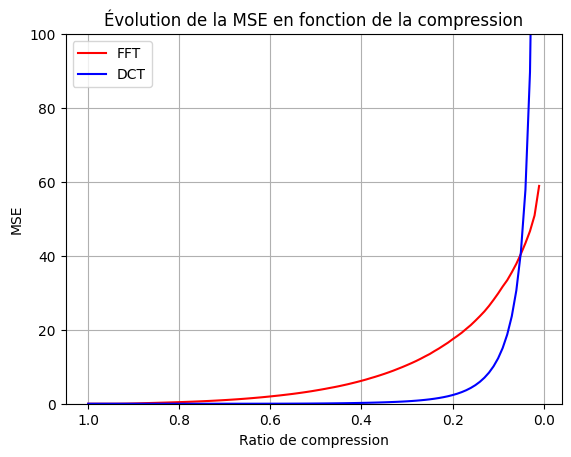
\includegraphics[width=0.5\textwidth]{images/MSE.png}
    \caption{Evolution de la MSE en fonction du ratio de la compression}
\end{figure}
On observe que la MSE sur l'image compressée avec la DCT est inférieure à la MSE de l'image compressée avec la FFT.

Cette métrique telle quelle est peu utilisée en traitement du signal mais sert souvent à calculer une autre métrique 
plus adaptée pour la quantification de la compression de signal.

\subsection{Peak Signal-to-Noise Ratio}

La métrique \textbf{Peak Signal-to-Noise Ratio (PSNR)} est la plus utilisée pour la compression d'images. Elle est basée sur le calcul de l'erreur moyenne quadratique.
\\ Le PSNR s'exprime en décibels dB.
$$ PSNR = 10 \cdot \log_{10}(\frac{255^2}{MSE})$$
Cette métrique donne le rapport entre la valeur maximale d'un pixel au carré et la MSE. Le passage au $\log_{10}$ et l'ajout du facteur $10$ permettent de réduire l'échelle 
des valeurs prises par le PSNR afin que cela soit plus facilement interprétable par une personne. Ainsi, une valeur très faible indique une perte conséquente de qualité d'image, alors
qu'une valeur élevée indique une image compressée fidèle à l'image originale.

\begin{figure}[H]
    \centering
    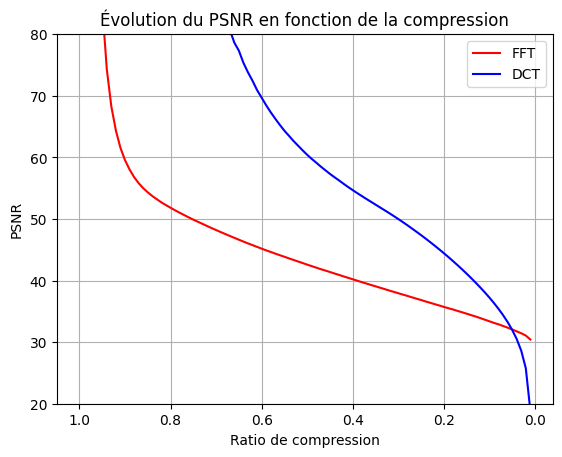
\includegraphics[width=0.5\textwidth]{images/PSNR.png}
    \caption{Evolution du PSNR en fonction du ratio de la compression}
\end{figure}

On observe logiquement que le PSNR est meilleur avec la DCT qu'avec la FFT car la MSE donnée après compression avec DCT était inférieure à la MSE après compression avec FFT.

Les deux métriques vues précédemment étant purement mathématiques, elles restent difficiles à interpréter. 
De plus, une valeur d'une métrique peut avoir plusieurs interprétations. Ainsi, une modification uniforme peut engendrer la même erreur que 
l'ajout d'un artéfact concentré en une région de l'image. Il peut alors devenir intéressant de développer de nouvelles métriques plus proches de la vision humaine.

\subsection{Structural Similarity Index Measure}

La \textbf{Structural Similarity Index Measure (SSIM)} se concentre sur la perception de l'oeil humain plutôt que sur la théorie mathématique. 
Contrairement à la MSE et au PSNR qui reposent sur des différences pixel à pixel, la SSIM compare la structure globale de l'image. Elle est calculée à l'aide de 
deux fenêtres de taille $N\times N$, la première ($x$) sur l'image originale et la seconde ($y$) sur l'image compressée : 
$$SSIM(x,y) = \frac{(2\mu_x\mu_y + c_1)(2\sigma_x\sigma_y+c_2)(\sigma_{xy}+c_3)}{(\mu_x^2+\mu_y^2+c_1)(\sigma_x^2+\sigma_y^2+c_2)(\sigma_x\sigma_y+c_3)}$$
avec :
\begin{itemize}
    \item $\mu_x$ : moyenne de $x \quad \mu_y$ : moyenne de $y \quad \sigma_x^2$ : variance de $x \quad \sigma_y^2$ : variance de $y$
    \item $\sigma_{xy}$ : covariance de $x$ et $y$
    \item $c_1 = (0.01\cdot 255)^2 = 6.5025 \quad c_2 = (0.03\cdot 255)^2 = 58.5225 \quad c_3 = \frac{c_2}{2} = 29.26125$
\end{itemize}
Les constantes $c_1$,$c_2$ et $c_3$ ont été établies en fonction des caractéristiques de la vision humaine.
Cette formule est construite en combinant trois rapports : la \textbf{luminance}, le \textbf{contraste} et la \textbf{structure}. \\
La \textbf{luminance} compare la luminosité moyenne entre les deux fenêtres : 
$$ l(x,y) = \frac{2\mu_x \mu_y + c_1}{\mu_x^2 + \mu_y^2 + c_1} $$
Ainsi, plus les moyennes sont proches, plus la luminance tend vers 1. Dans le cas contraire, plus les moyennes s'éloignent, plus la luminance diminue vers $0$. \\
Le \textbf{contraste} compare l'amplitude des variations de lumière sur les deux fenêtres : 
$$ c(x,y) = \frac{2\sigma_x \sigma_y + c_2}{\sigma_x^2 + \sigma_y^2 + c_2} $$
Plus les variances sont proches, plus le contraste tend vers 1. Dans le cas contraire, plus les variances s'éloignent, plus le contraste diminue vers $0$. \\
La \textbf{structure} compare la corrélation entre les deux fenêtres :
$$ s(x,y) = \frac{cov_{xy}+c_3}{\sigma_x\sigma_y+c_3} $$
Si on omet la constante $c_3$, on reconnait ici le coefficient de corrélation de Pearson. Il mesure la direction d'une relation linéaire entre deux variables. 
Plus le coefficient de corrélation est proche de 1, plus les variables suivent une même trajectoire. \\
Finalement, on obtient :
$$ SSIM(x,y) = l(x,y) \cdot c(x,y) \cdot s(x,y) $$
Ainsi, plus la luminance, le contraste et la structure sont semblables entre les deux images, plus chaque rapport tend vers $1$.
On en déduit que plus la SSIM est proche de $1$ et plus les images sont semblables entre elles.

\begin{figure}[H]
    \centering
    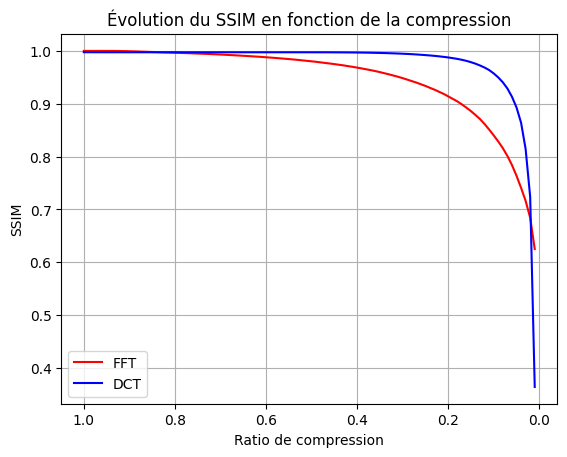
\includegraphics[width=0.5\textwidth]{images/SSIM.png}
    \caption{Evolution du SSIM en fonction du ratio de la compression}
\end{figure}
On observe que la SSIM est bien meilleure avec la DCT qu'avec la FFT. On peut expliquer cela car la DCT regroupe les zones sans détails en carrés et garde
les zones détaillées nettes. Ainsi, les zones plus détaillées sont peu modifiées alors que le fond de l'image qui est moins détaillé devient flou au fil de la compression, modifiant peu la perception finale de l'image.

